% Source PDF page 623 (printed p. 609)
\section{原始—对偶内点法}
本节介绍一种基本的原始—对偶内点法。原始—对偶内点法与障碍法很相似，但有如下区别。
\begin{itemize}
\item 只有一层循环或迭代，不像障碍法那样区分内迭代和外迭代。每次迭代同时更新原始变量与对偶变量。
\item 原始—对偶内点法对修改后的 KKT 方程，即对数障碍中心化问题的最优性条件，应用牛顿法得到搜索方向。原始—对偶搜索方向与障碍法产生的搜索方向相似，但并不完全相同。
\item 原始—对偶内点法的原始迭代点和对偶迭代点不一定可行。
\end{itemize}
原始—对偶内点法通常比障碍法更有效，特别是在要求高精度时，因为它们可以表现出快于线性的收敛速度。对线性规划、二次规划、二阶锥规划、几何规划和半定规划等几类基本问题，专门设计的原始—对偶方法优于障碍法。对一般非线性凸优化问题，原始—对偶内点法仍是活跃的研究课题，但前景很好。它相对障碍法的另一个优点，是在问题可行但不严格可行时也能工作，不过这里不再深入讨论。

本节给出求解 (11.1) 的一种基本原始—对偶方法，不作收敛性分析。关于原始—对偶方法及其收敛性分析的更全面论述，请参阅参考文献。

\subsection{原始—对偶搜索方向}
与障碍法一样，从修改后的 KKT 条件 (11.15) 出发，将其写为 $r_t(x,\lambda,\nu)=0$，其中定义
\begin{equation}
r_t(x,\lambda,\nu)=\begin{bmatrix}
\nabla f_0(x)+Df(x)^\T\lambda+A^\T\nu\\
-\diag(\lambda)f(x)-(1/t)\one\\
Ax-b
\end{bmatrix},\tag{11.53}
\end{equation}
且 $t>0$。这里 $f:\R^n\to\R^m$ 及其导数矩阵 $Df$ 为
\[
f(x)=\begin{bmatrix}f_1(x)\\\vdots\\f_m(x)\end{bmatrix},\qquad
Df(x)=\begin{bmatrix}\nabla f_1(x)^\T\\\vdots\\\nabla f_m(x)^\T\end{bmatrix}.
\]
若 $x,\lambda,\nu$ 满足 $r_t(x,\lambda,\nu)=0$，且 $f_i(x)<0$，则 $x=x^\star(t)$、$\lambda=\lambda^\star(t)$、$\nu=\nu^\star(t)$。特别地，$x$ 原始可行，$\lambda,\nu$ 对偶可行，
% Source PDF page 624 (printed p. 610)
对偶间隙为 $m/t$。$r_t$ 的第一个分块
\[
r_{\mathrm{dual}}=\nabla f_0(x)+Df(x)^\T\lambda+A^\T\nu
\]
称为\emph{对偶残差}，最后一个分块 $r_{\mathrm{pri}}=Ax-b$ 称为\emph{原始残差}。中间分块
\[
r_{\mathrm{cent}}=-\diag(\lambda)f(x)-(1/t)\one
\]
是\emph{中心性残差}，即修改后互补条件的残差。

现在固定 $t$，在满足 $f(x)\prec0$、$\lambda\succ0$ 的点 $(x,\lambda,\nu)$ 处，考虑求解非线性方程 $r_t(x,\lambda,\nu)=0$ 的牛顿步，不像第11.3.4节那样预先消去 $\lambda$。分别将当前点和牛顿步记为
\[
y=(x,\lambda,\nu),\qquad\Delta y=(\Delta x,\Delta\lambda,\Delta\nu).
\]
牛顿步由线性方程
\[
r_t(y+\Delta y)\approx r_t(y)+Dr_t(y)\Delta y=0
\]
刻画，即 $\Delta y=-Dr_t(y)^{-1}r_t(y)$。用 $x,\lambda,\nu$ 表示，得到
\begin{equation}
\begin{bmatrix}
\nabla^2 f_0(x)+\sum_{i=1}^m\lambda_i\nabla^2 f_i(x)&Df(x)^\T&A^\T\\
-\diag(\lambda)Df(x)&-\diag(f(x))&0\\
A&0&0
\end{bmatrix}
\begin{bmatrix}\Delta x\\\Delta\lambda\\\Delta\nu\end{bmatrix}
=-\begin{bmatrix}r_{\mathrm{dual}}\\r_{\mathrm{cent}}\\r_{\mathrm{pri}}\end{bmatrix}.
\tag{11.54}
\end{equation}
\emph{原始—对偶搜索方向} $\Delta y_{\mathrm{pd}}=(\Delta x_{\mathrm{pd}},\Delta\lambda_{\mathrm{pd}},\Delta\nu_{\mathrm{pd}})$ 定义为 (11.54) 的解。

原始搜索方向和对偶搜索方向通过系数矩阵与残差相互耦合。例如，原始搜索方向 $\Delta x_{\mathrm{pd}}$ 既依赖 $x$，也依赖当前对偶变量 $\lambda,\nu$。还应注意，若 $x$ 满足 $Ax=b$，即原始可行性残差 $r_{\mathrm{pri}}$ 为零，则 $A\Delta x_{\mathrm{pd}}=0$，所以 $\Delta x_{\mathrm{pd}}$ 是原始可行方向：对任意 $s$，$x+s\Delta x_{\mathrm{pd}}$ 都满足 $A(x+s\Delta x_{\mathrm{pd}})=b$。

\subsubsection*{与障碍法搜索方向的比较}
原始—对偶搜索方向与障碍法使用的搜索方向关系密切，但并不完全相同。从定义原始—对偶搜索方向的线性方程 (11.54) 出发，利用第二组分块方程给出的
\[
\Delta\lambda_{\mathrm{pd}}=-\diag(f(x))^{-1}\diag(\lambda)Df(x)\Delta x_{\mathrm{pd}}
+\diag(f(x))^{-1}r_{\mathrm{cent}},
\]
消去变量 $\Delta\lambda_{\mathrm{pd}}$。将它代入第一组分块方程，得到
\begin{equation}\begin{aligned}
\begin{bmatrix}H_{\mathrm{pd}}&A^\T\\A&0\end{bmatrix}
\begin{bmatrix}\Delta x_{\mathrm{pd}}\\\Delta\nu_{\mathrm{pd}}\end{bmatrix}
&=-\begin{bmatrix}r_{\mathrm{dual}}+Df(x)^\T\diag(f(x))^{-1}r_{\mathrm{cent}}\\r_{\mathrm{pri}}\end{bmatrix}\\
&=-\begin{bmatrix}\nabla f_0(x)+(1/t)\sum_{i=1}^m\frac1{-f_i(x)}\nabla f_i(x)+A^\T\nu\\r_{\mathrm{pri}}\end{bmatrix},
\end{aligned}\tag{11.55}\end{equation}
% Source PDF page 625 (printed p. 611)
其中
\begin{equation}
H_{\mathrm{pd}}=\nabla^2 f_0(x)+\sum_{i=1}^m\lambda_i\nabla^2 f_i(x)
+\sum_{i=1}^m\frac{\lambda_i}{-f_i(x)}\nabla f_i(x)\nabla f_i(x)^\T.\tag{11.56}
\end{equation}
将 (11.55) 与方程 (11.14) 比较，后者定义了障碍法参数为 $t$ 时中心化问题的牛顿步。它可以写为
\begin{equation}\begin{aligned}
\begin{bmatrix}H_{\mathrm{bar}}&A^\T\\A&0\end{bmatrix}
\begin{bmatrix}\Delta x_{\mathrm{bar}}\\\nu_{\mathrm{bar}}\end{bmatrix}
&=-\begin{bmatrix}t\nabla f_0(x)+\nabla\phi(x)\\r_{\mathrm{pri}}\end{bmatrix}\\
&=-\begin{bmatrix}t\nabla f_0(x)+\sum_{i=1}^m\frac1{-f_i(x)}\nabla f_i(x)\\r_{\mathrm{pri}}\end{bmatrix},
\end{aligned}\tag{11.57}\end{equation}
其中
\begin{equation}
H_{\mathrm{bar}}=t\nabla^2 f_0(x)+\sum_{i=1}^m\frac1{-f_i(x)}\nabla^2 f_i(x)
+\sum_{i=1}^m\frac1{f_i(x)^2}\nabla f_i(x)\nabla f_i(x)^\T.\tag{11.58}
\end{equation}
这里给出了不可行牛顿步的一般表达式。若当前 $x$ 可行，即 $r_{\mathrm{pri}}=0$，则 $\Delta x_{\mathrm{bar}}$ 与 (11.14) 定义的可行牛顿步 $\Delta x_{\mathrm{nt}}$ 一致。

首先，两个方程组 (11.55) 和 (11.57) 非常相似。它们的系数矩阵具有相同结构：$H_{\mathrm{pd}}$ 与 $H_{\mathrm{bar}}$ 都是矩阵
\[
\nabla^2 f_0(x),\quad\nabla^2 f_1(x),\ldots,\nabla^2 f_m(x),\quad
\nabla f_1(x)\nabla f_1(x)^\T,\ldots,\nabla f_m(x)\nabla f_m(x)^\T
\]
的正线性组合。这意味着可以用同一种方法计算原始—对偶搜索方向和障碍法牛顿步。

关于原始—对偶方程 (11.55) 与障碍法方程 (11.57) 的关系，还可以进一步说明。将 (11.57) 第一组分块方程除以 $t$，并定义变量 $\Delta\nu_{\mathrm{bar}}=(1/t)\nu_{\mathrm{bar}}-\nu$，其中 $\nu$ 任意，得到
\[
\begin{bmatrix}(1/t)H_{\mathrm{bar}}&A^\T\\A&0\end{bmatrix}
\begin{bmatrix}\Delta x_{\mathrm{bar}}\\\Delta\nu_{\mathrm{bar}}\end{bmatrix}
=-\begin{bmatrix}\nabla f_0(x)+(1/t)\sum_{i=1}^m\frac1{-f_i(x)}\nabla f_i(x)+A^\T\nu\\r_{\mathrm{pri}}\end{bmatrix}.
\]
这个形式的右端与在相同 $x,\lambda,\nu$ 处计算的原始—对偶方程右端一致。系数矩阵仅在 $(1,1)$ 分块有所不同：
\begin{align*}
H_{\mathrm{pd}}&=\nabla^2 f_0(x)+\sum_{i=1}^m\lambda_i\nabla^2 f_i(x)
+\sum_{i=1}^m\frac{\lambda_i}{-f_i(x)}\nabla f_i(x)\nabla f_i(x)^\T,\\
(1/t)H_{\mathrm{bar}}&=\nabla^2 f_0(x)+\sum_{i=1}^m\frac1{-tf_i(x)}\nabla^2 f_i(x)
+\sum_{i=1}^m\frac1{tf_i(x)^2}\nabla f_i(x)\nabla f_i(x)^\T.
\end{align*}
当 $x$ 与 $\lambda$ 满足 $-f_i(x)\lambda_i=1/t$ 时，系数矩阵相同，搜索方向因而也相同。

% Source PDF page 626 (printed p. 612)
\subsection{代理对偶间隙}
原始—对偶内点法中的迭代点 $x^{(k)},\lambda^{(k)},\nu^{(k)}$ 不一定可行，只有算法收敛的极限点才可行。这意味着，无法像障碍法的外迭代那样，容易地计算算法第 $k$ 步对应的对偶间隙 $\eta^{(k)}$。取而代之，对于任意满足 $f(x)\prec0$、$\lambda\succeq0$ 的 $x,\lambda$，定义\emph{代理对偶间隙}
\begin{equation}
\widehat\eta(x,\lambda)=-f(x)^\T\lambda.\tag{11.59}
\end{equation}
如果 $x$ 原始可行、$\lambda,\nu$ 对偶可行，即 $r_{\mathrm{pri}}=0$、$r_{\mathrm{dual}}=0$，则代理间隙 $\widehat\eta$ 就是对偶间隙。注意，与代理对偶间隙 $\widehat\eta$ 对应的参数 $t$ 为 $m/\widehat\eta$。

\subsection{原始—对偶内点法}
现在可以给出基本原始—对偶内点算法。

\begin{origalgorithm}{11.2}
\textbf{原始—对偶内点法。}

给定满足 $f_1(x)<0,\ldots,f_m(x)<0$ 的 $x$，以及 $\lambda\succ0$、$\mu>1$、$\epsilon_{\mathrm{feas}}>0$、$\epsilon>0$。

重复：
\begin{enumerate}
\item \textbf{确定 $t$。} 取 $t:=\mu m/\widehat\eta$。
\item \textbf{计算原始—对偶搜索方向} $\Delta y_{\mathrm{pd}}$。
\item \textbf{线搜索与更新。} 确定步长 $s>0$，取 $y:=y+s\Delta y_{\mathrm{pd}}$。
\end{enumerate}
直至 $\norm{r_{\mathrm{pri}}}_2\le\epsilon_{\mathrm{feas}}$、$\norm{r_{\mathrm{dual}}}_2\le\epsilon_{\mathrm{feas}}$，并且 $\widehat\eta\le\epsilon$。
\end{origalgorithm}
第1步把参数 $t$ 设为 $m/\widehat\eta$ 的 $\mu$ 倍，其中 $m/\widehat\eta$ 是与当前代理对偶间隙对应的 $t$ 值。若 $x,\lambda,\nu$ 是参数 $t$ 对应的中心点，因而对偶间隙为 $m/t$，则第1步将 $t$ 增大 $\mu$ 倍，这与障碍法的更新完全相同。参数 $\mu$ 取约为 $10$ 的值似乎效果很好。

当 $x$ 原始可行、$\lambda,\nu$ 对偶可行（容差内，容差为 $\epsilon_{\mathrm{feas}}$），并且代理间隙小于容差 $\epsilon$ 时，原始—对偶内点算法终止。由于原始—对偶内点法经常快于线性收敛，通常会取较小的 $\epsilon_{\mathrm{feas}}$ 与 $\epsilon$。

\subsubsection*{线搜索}
原始—对偶内点法采用基于残差范数的标准回溯线搜索，并作修改以保证 $\lambda\succ0$、$f(x)\prec0$。当前迭代点记为 $x,\lambda,\nu$，下一迭代点记为 $x^+,\lambda^+,\nu^+$，即
\[
x^+=x+s\Delta x_{\mathrm{pd}},\qquad
\lambda^+=\lambda+s\Delta\lambda_{\mathrm{pd}},\qquad
\nu^+=\nu+s\Delta\nu_{\mathrm{pd}}.
\]
% Source PDF page 627 (printed p. 613)
在 $y^+$ 处计算的残差记为 $r^+$。

首先计算不超过 $1$ 且使 $\lambda^+\succeq0$ 的最大正步长，即
\begin{align*}
s_{\mathrm{max}}&=\sup\{s\in[0,1]\mid\lambda+s\Delta\lambda\succeq0\}\\
&=\min\bigl\{1,\min\{-\lambda_i/\Delta\lambda_i\mid\Delta\lambda_i<0\}\bigr\}.
\end{align*}
回溯从 $s=0.99s_{\mathrm{max}}$ 开始，反复将 $s$ 乘以 $\beta\in(0,1)$，直至 $f(x^+)\prec0$。继续将 $s$ 乘以 $\beta$，直至
\[
\norm{r_t(x^+,\lambda^+,\nu^+)}_2\le(1-\alpha s)\norm{r_t(x,\lambda,\nu)}_2.
\]
回溯参数 $\alpha,\beta$ 的常见取法与牛顿法相同：$\alpha$ 通常在 $0.01$ 至 $0.1$ 之间，$\beta$ 通常在 $0.3$ 至 $0.8$ 之间。

原始—对偶内点算法的一次迭代，相当于不可行牛顿法为求解 $r_t(x,\lambda,\nu)=0$ 而执行的一步，只是修改为保证 $\lambda\succ0$、$f(x)\prec0$；等价地，将 $r_t$ 的定义域限制为 $\lambda\succ0$、$f(x)\prec0$。用不可行初始点牛顿法收敛性证明中的相同论证，可以说明原始—对偶方法的线搜索总在有限步内终止。

\subsection{例子}
用第11.3.2节的相同问题展示原始—对偶内点法的性能。唯一区别是，这里不像第11.3.2节那样从中心路径上的点出发，而是随机生成满足 $f(x)\prec0$ 的 $x^{(0)}$，并取 $\lambda_i^{(0)}=-1/f_i(x^{(0)})$，因此初始代理间隙为 $\widehat\eta=100$。使用的原始—对偶内点法参数为
\[
\mu=10,\qquad\beta=0.5,\qquad\epsilon=10^{-8},\qquad\alpha=0.01.
\]

\subsubsection*{小型 LP 与 GP}
首先考虑第11.3.2节的小型 LP，包含 $m=100$ 个不等式和 $n=50$ 个变量。图11.21展示原始—对偶内点法的进展，给出了代理间隙 $\widehat\eta$ 和原始、对偶残差范数
\[
r_{\mathrm{feas}}=\left(\norm{r_{\mathrm{pri}}}_2^2+\norm{r_{\mathrm{dual}}}_2^2\right)^{1/2}
\]
随迭代次数变化的两条曲线。初始点原始可行，所以图中反映的是对偶可行性残差的范数。曲线表明，残差迅速趋于零，$24$ 次迭代后在数值精度范围内为零。代理间隙也迅速收敛。与障碍法相比，原始—对偶内点法更快，特别是在要求高精度时。

图11.22给出了原始—对偶内点法求解第11.3.2节 GP 的进展，收敛情况与 LP 相似。

% Source PDF page 628 (printed p. 614)
\begin{figure}[htbp]\centering
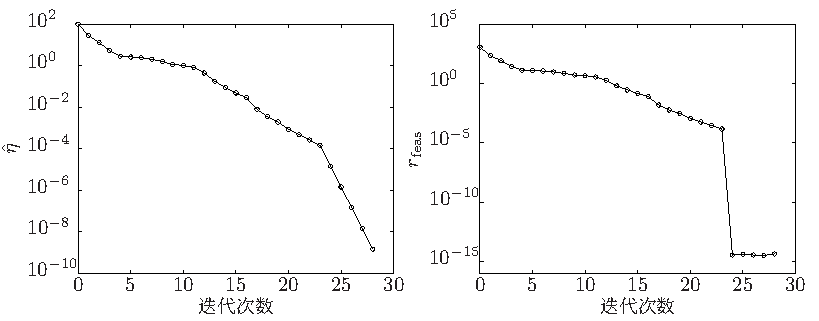
\includegraphics[width=.95\textwidth]{figures/ch11-21.pdf}
\caption*{图11.21 原始—对偶内点法求解 LP 的进展：代理对偶间隙 $\widehat\eta$ 以及原始、对偶残差范数与迭代次数的关系。残差在 $24$ 次迭代内迅速收敛到零；代理间隙也在约 $28$ 次迭代后收敛到很小的值。原始—对偶内点法比障碍法收敛更快，特别是在要求高精度时。}
\end{figure}
\begin{figure}[htbp]\centering
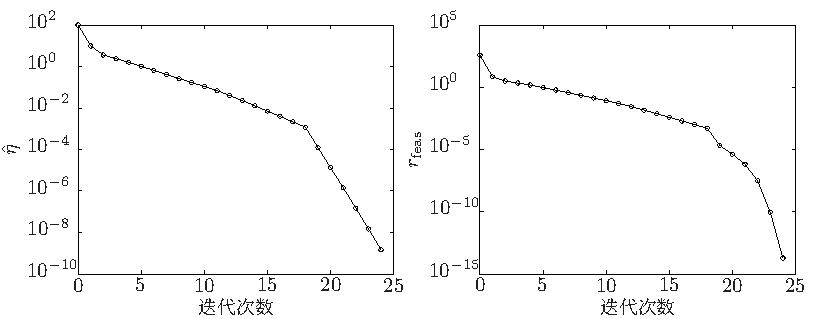
\includegraphics[width=.95\textwidth]{figures/ch11-22.pdf}
\caption*{图11.22 原始—对偶内点法求解 GP 的进展：代理对偶间隙 $\widehat\eta$ 以及原始、对偶残差范数与迭代次数的关系。}
\end{figure}

% Source PDF page 629 (printed p. 615)
\begin{figure}[htbp]\centering
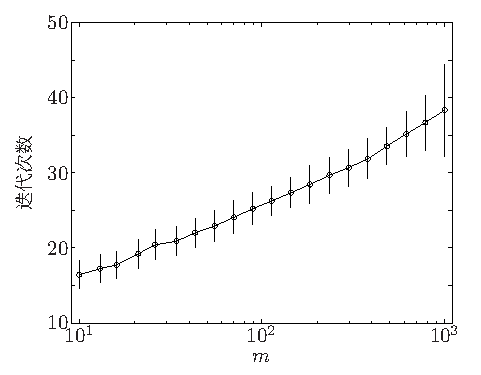
\includegraphics[width=.6\textwidth]{figures/ch11-23.pdf}
\caption*{图11.23 求解不同维数随机标准 LP 所需的迭代次数，$n=2m$。误差棒给出每个维数的 $100$ 个实例中围绕均值的标准差。问题维数变化 $100$ 倍时，所需迭代次数近似按对数增长。}
\end{figure}

\subsubsection*{一族 LP}
这里使用第11.3.2节相同的一族标准形式 LP，考察原始—对偶方法的性能与问题维数的关系。用原始—对偶内点法求解同样的 $2000$ 个实例，每个 $m$ 值对应 $100$ 个实例。算法从 $x^{(0)}=\one$、$\lambda^{(0)}=\one$、$\nu^{(0)}=0$ 出发，终止容差为 $\epsilon=10^{-8}$。图11.23给出所需迭代次数的均值与标准差随 $m$ 的变化。迭代次数从 $15$ 到 $35$，近似随 $m$ 的对数增长。与图11.8的障碍法结果比较可见，尽管我们从不可行初始点出发，并将问题求到高得多的精度，原始—对偶方法的迭代次数也只略多一些。
